\message{ !name(ELP1P1.tex)}\documentclass{article}

\usepackage{circuitikz} %Für die Schaltpläne
\usepackage[T1]{fontenc} 
\usepackage[utf8]{inputenc}
\usepackage{amsmath}
\usepackage{amssymb}
\usepackage{fancyhdr}
\usepackage{graphicx}
\usepackage{hyperref}
\usepackage{subcaption}
\usepackage{tikz}
\usepackage{../assets/scripts/tex/color-env}
\usepackage[ngerman]{babel}



    \usetikzlibrary{arrows}
    \usetikzlibrary{arrows.meta,topaths}
    \usetikzlibrary{bending}
    \usetikzlibrary{calc}
\title{Elektrotechnik 1 Praktikum 1}


\usepackage[
  includehead,
  headheight = 17mm,
  footskip = \dimexpr\headsep+\ht\strutbox\relax,
  tmargin = 0mm,
  bmargin = \dimexpr17mm+2\ht\strutbox\relax,
]{geometry}

\usepackage{anyfontsize}

\usepackage{xcolor}

\definecolor{DarkGreenBlue}{HTML}{264653}
\definecolor{LightGreenBlue}{HTML}{2A9D8F}
\definecolor{LightOrange}{HTML}{E9C46A}
\definecolor{DarkOrange}{HTML}{F4A261}
\definecolor{RedOrange}{HTML}{E76F51}
\definecolor{BrightRed}{HTML}{D62828}
\definecolor{DeepBlue}{HTML}{003049}



\pagestyle{fancy}
\fancyhead[L]{\leftmark}
\fancyhead[R]{}
\fancyfoot[L]{}
\fancyfoot[C]{\thepage}
\fancyfoot[R]{
\includegraphics[scale=0.2]{../assets/images/haw.jpg}}
\renewcommand\headrulewidth{0.5pt}


\begin{document}

\message{ !name(ELP1P1.tex) !offset(115) }
    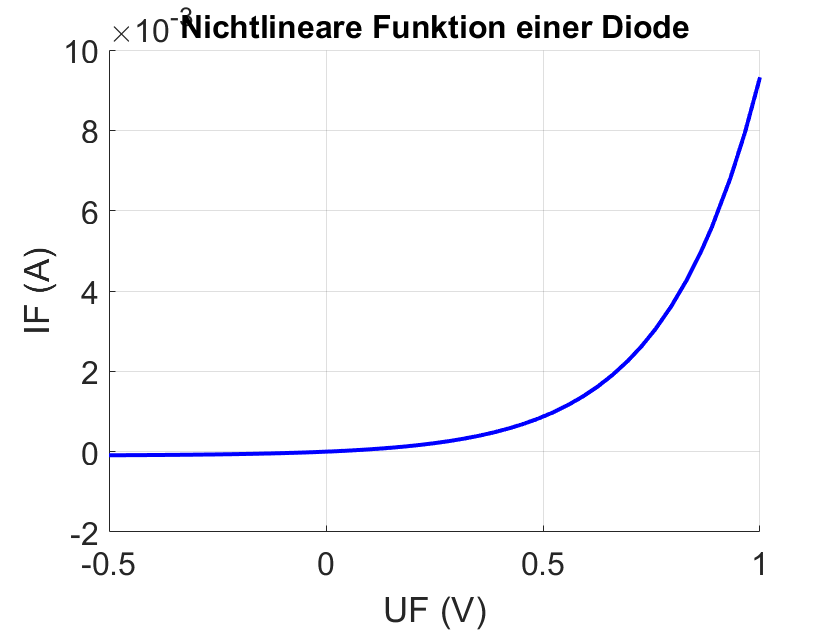
\includegraphics[width=\textwidth]{../assets/images/EL1P2/VorbereitungAA138.png}
    \caption{Kennlinie der AA138 Germaniumdiode}
  \end{subfigure}
  \hfill
  \begin{subfigure}[b]{0.4\textwidth}
    \centering
    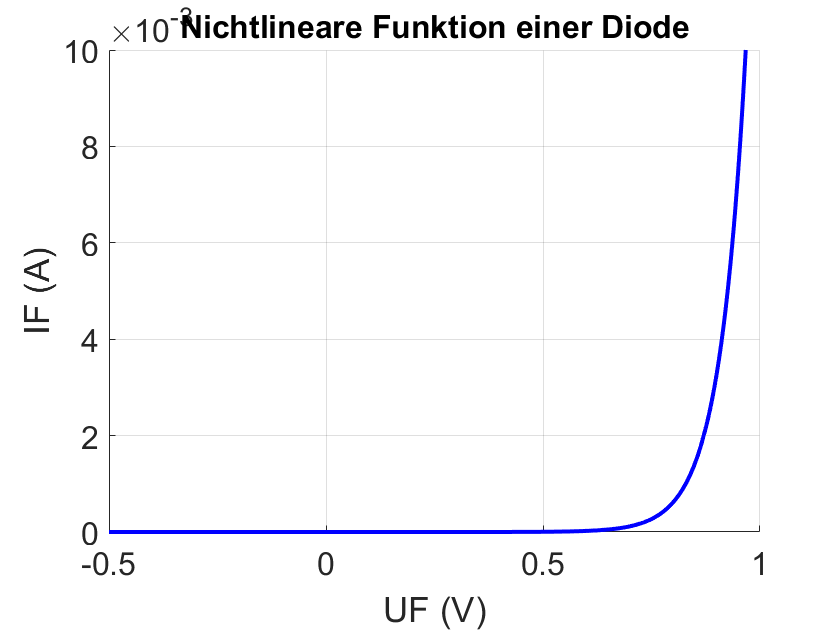
\includegraphics[width=\textwidth]{../assets/images/EL1P2/Vorbereitung1N4148.png}
    \caption{Kennlinie der 1N4148 Siliziumdiode}
  \end{subfigure}
  \caption{Die beiden Kennlinien der Dioden simuliert mit Shockley in Matlab}
\end{figure}

\subsection{Versuchsdurchführung}

Wir messen mithilfe des X-Y-Schreibers, wie im Versuchsaufbau gezeigt, den Strom über die Diode indirekt mithilfe der Spannung 
über den Vorwiderstand (Shunt). Die Spannung über die Diode messen wir einfach direkt mit den X-Eingängen des Schreibers. Den Strom durch den Schaltkreis regeln wir bis zu einem Stromfluss von 10mA hoch und nehmen dabei die 
Kennlinie der jeweiligen Diode auf.
\newpage
\subsection{Auswertung}

Wir legen an die Kennlinien jeweils eine Tangente an die Stelle $y=2mA$ und bestimmen daraus die Steigung und damit den differentiellen Widerstand der Diode:
\begin{figure}[h]
  \centering
  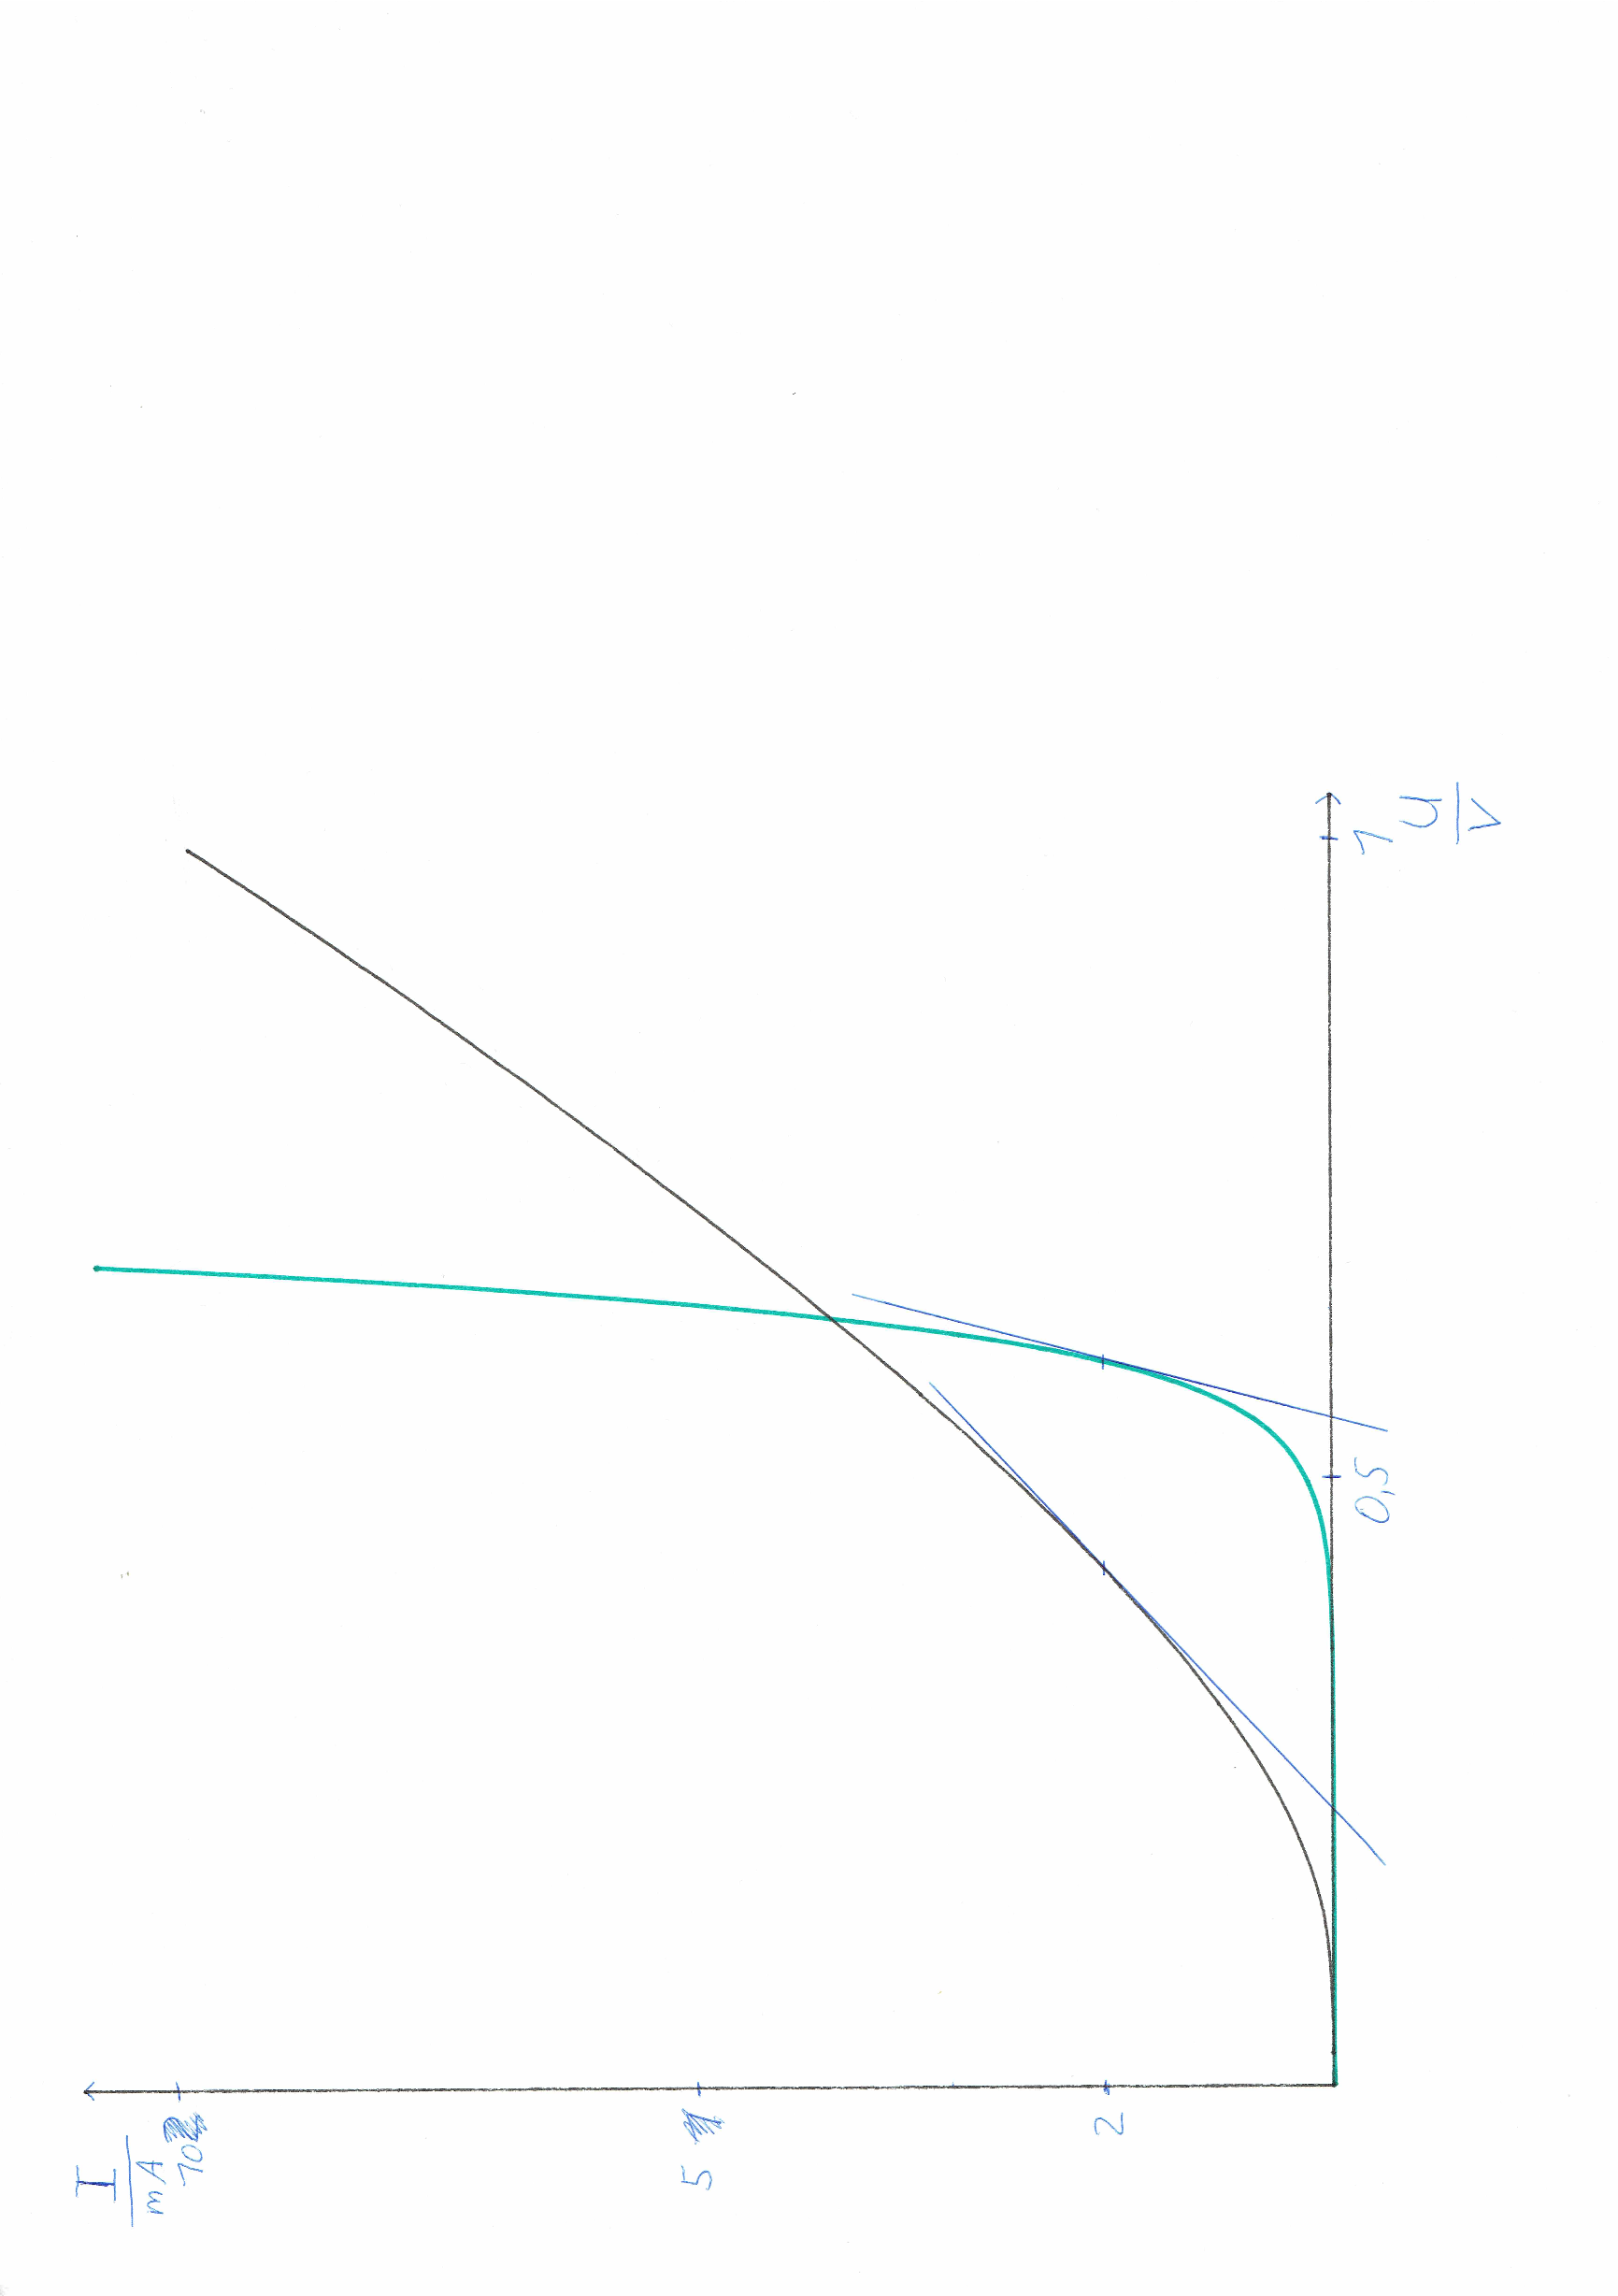
\includegraphics[scale=0.4, angle=-90]{../assets/images/EL1P2/ScanXY.PDF}
  \caption{Ergebnis des Aufnehmen der Kennlinie mit dem XY-Schreiber. (Blau 1N4148, Schwarz AA138)}
  \label{fig:xy}
\end{figure}

Wir erkennen, dass die Diodenkennlinie der Siliziumdiode um einiges stärker definiert ist und ihre Vorwärtspannung ab einem bestimmten Punkt einen stark expotentiellen Verlauf annimmt. Das ist auch mit ein Grund, warum Germaniumdioden heutzutage einen weitaus geringeren Stellenwert haben als Siliziumdioden, da sich Siliziumdioden besser vorhersagen und am Computer quantisieren lassen. Für die Siliziumdiode erhalten wir einen differentiellen Widerstand von $G_{Si_{d}}= \frac{2mA-0,2mA}{0,6V-0,5V} = \frac{1,8mA}{0,1V} = 0,018S$, also $r_{Si_{r}} = \frac{1}{G_{Si_{d}}} = \frac{1}{0,018S} = 55,5\Omega$. Für die Germaniumdiode bekommen wir mit der Grafik nun

\message{ !name(ELP1P1.tex) !offset(290) }

\end{document}
